\documentclass[10pt,a4paper]{article}
\usepackage[utf8]{inputenc}
\usepackage[T1]{fontenc}
\usepackage{amsmath}
\usepackage{amsfonts}
\usepackage{amssymb}
\usepackage{graphicx}
\def\figurename{Figura}

\author{Daniel Walther Berns}
\title{Como trabajar en pythonanywhere}

\begin{document}
\section{Como pasar programas a pythonanywhere}

\subsection{Crear un directorio para los repositorios}

\begin{enumerate}
	\item En la pantalla Dashboard o panel de control de pythonanywhere, abrir una consola bash.
	\item Ejecutar los siguientes comandos en la consola:
	\begin{enumerate}
		\item Para asegurarnos que estamos en el directorio raíz
		\begin{verbatim}
$ cd ~
		\end{verbatim}
	    \item Creamos el directorio Code (código en inglés)
	    \begin{verbatim}
$ mkdir Code
	    \end{verbatim}
	    \item Entramos en el directorio Code (código en inglés)
        \begin{verbatim}
$ cd Code
        \end{verbatim}
    \item Vemos el path o camino,
\begin{verbatim}
$ pwd
\end{verbatim}
que debería ser similar a
\begin{verbatim}
/home/usuario_pythonanywhere/Code/
\end{verbatim}    

	\end{enumerate}
\end{enumerate}

\subsection{Como clonar un repositorio de Github}

\begin{enumerate}
	\item Obtener la dirección del repositorio (ver figura \ref{fig:urlrepo})
    \item Dashboard o panel de control de pythonanywhere, abrir una consola bash.
	\item Ejecutar los siguientes comandos en la consola:
    \begin{enumerate}
	\item Para asegurarnos que estamos en el directorio Code
	\begin{verbatim}
$ cd ~/Code
	\end{verbatim}
	\item Clonamos el repo
	\begin{verbatim}
$ git clone https://github.com/usuario_github/nombrerepo.git
	\end{verbatim}
	\item Entramos en el repo
	\begin{verbatim}
$ cd nombrerepo
	\end{verbatim}
    \item Vemos el path o camino,
    \begin{verbatim}
$ pwd
    \end{verbatim}
    que debería ser similar a
    \begin{verbatim}
$ /home/usuario_pythonanywhere/Code/nombrerepo
    \end{verbatim}    
    \item Si no vemos este camino, podemos solucionarlo con
    \begin{verbatim}
$ cd ~/Code/nombrerepo
    \end{verbatim}
    \item Una vez dentro del directorio del repo, podemos ver los archivos con el comando
    \begin{verbatim}
$ ls
    \end{verbatim}
    \end{enumerate}
\end{enumerate}

\begin{figure}
	\centering
	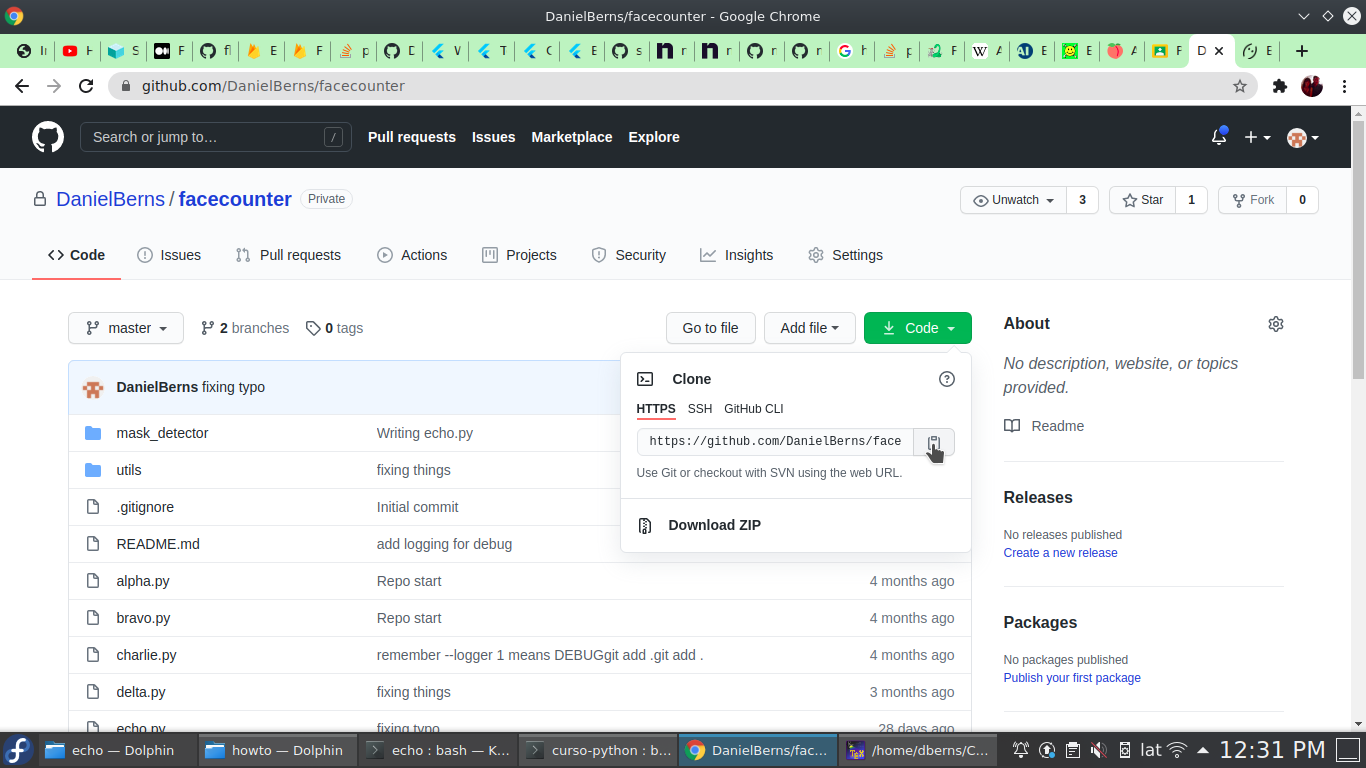
\includegraphics[width=1\linewidth]{sc/url_repo}
	\caption{Donde está url repo}
	\label{fig:urlrepo}
\end{figure}

\subsection{Como actualizar los repositorios en pythonanywhere}

No nos conviene modificar los archivos de los repositorios en pythonanywhere, porque los editores
son un tanto incómodos. Si quiere verificarlo, pruebe
\begin{verbatim}
$ vi test.txt
\end{verbatim}
No pregunte nada sobre este punto en el foro. ¡No recibirá respuesta!

Por lo tanto, nos conviene modificar los archivos en nuestras computadoras, actualizar el repositorio en Github y 
y después actualizar el repositorio en pythonanywhere. 

Si en sus computadoras están trabajando con Windows y Visual Studio pueden manejar la actualización del repositorio en Github con Visual Studio. Esto se explica en otro apunte y video. 

También es posible usar la página del repo en Github (ver figura \ref{fig:uploadfile}). Como vemos, podemos subir archivos directamente al repositorio. Es una forma lenta pero segura y simple si no se cuenta con un cliente de Git.

\begin{figure}
	\centering
	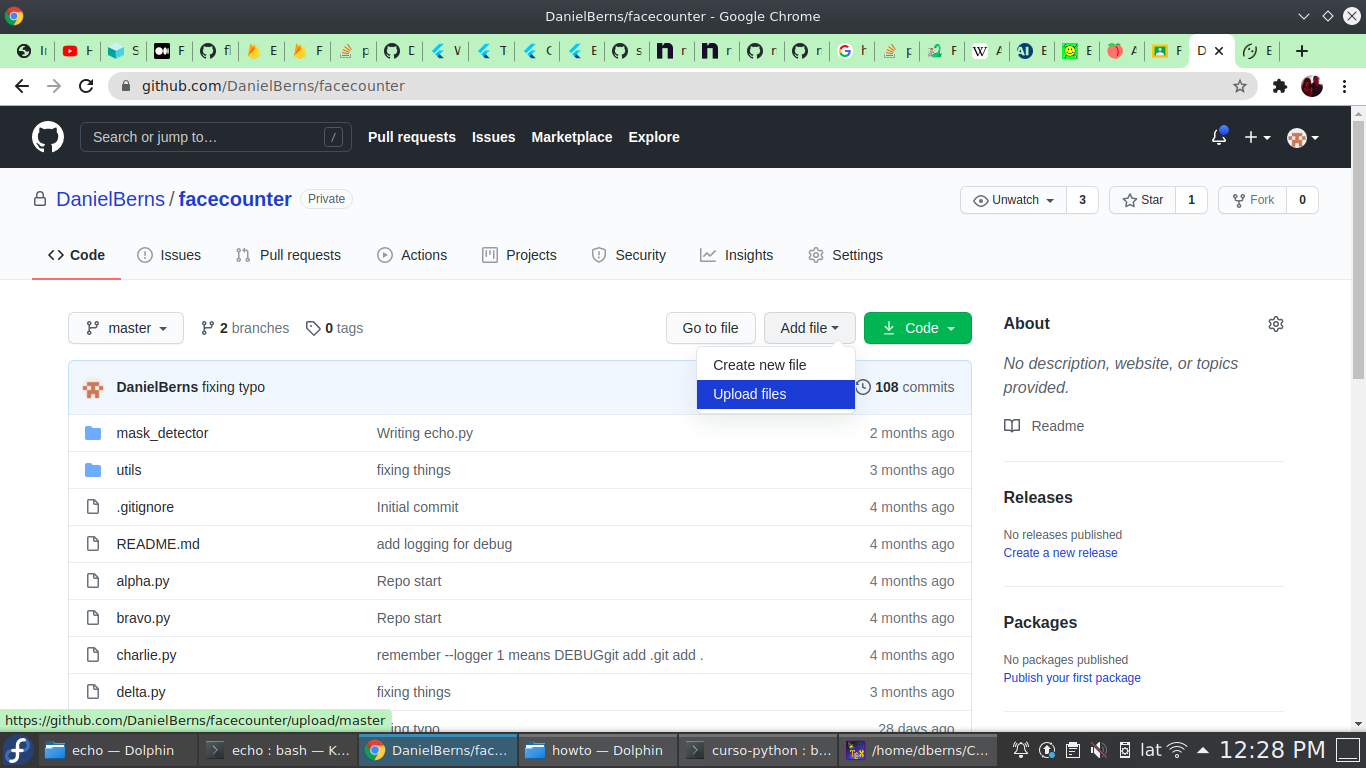
\includegraphics[width=1\linewidth]{sc/upload_file}
	\caption{Como subir archivos en la página del repositorio}
	\label{fig:uploadfile}
\end{figure}

Finalmente, para actualizar el repositorio en pythonanywhere, en el Dashboard o panel de control de pythonanywhere abrirmos una consola bash y ejecutamos los siguientes comandos:
\begin{enumerate}
	\item \begin{verbatim}
$ cd ~/Code/nombrerepo
	\end{verbatim}
    \item \begin{verbatim}
$ git pull
    \end{verbatim}
\end{enumerate}

\section{Como pasar archivos grandes a pythonanywhere}

Supongamos que necesitamos transferir a pythonanywhere archivos binarios grandes (fotografías, planillas excel, bases de datos, etc), desde Google Drive o Dropbox. Suponemos también que tenemos los enlace de acceso a dichos archivos. 

En el Dashboard o panel de control de pythonanywhere abrirmos una consola bash y ejecutamos el
siguiente comando
\begin{verbatim}
$ wget -O test.pdf link
\end{verbatim}
donde debemos reemplazar link por
\begin{verbatim}
https://drive.google.com/file/d/1HVBDQzbMmDPO5rmGFe65eI7Jlx--_BmZ/view?usp=sharing
\end{verbatim}

Si ejecutamos el comando ls, debemos ver como resultado el archivo \verb|test.pdf|.


\section{Como extraer archivos desde pythonanywhere}

Si ya clonaron el repositorio de este curso, pueden ver que en el directorio
\begin{verbatim}
curso-python/pythonanywhere/calendar/calendars
\end{verbatim}
hay un archivo html y dos directorios con más archivos html generados por el programa \verb|generate_two_hundred_years.py|. ¿Cómo podemos hacer para que estos archivos sean accesibles por Internet?

\subsection{Crear una aplicación web en pythonanywhere}

En la pantalla Dashboard aparece un enlace con el título Web (figura \ref{fig:webappdashboard}). Si seguimos ese enlace vamos a la pantalla Web donde podemos crear una aplicación web (figura \ref{fig:webappcreate}).

\begin{figure}
	\centering
	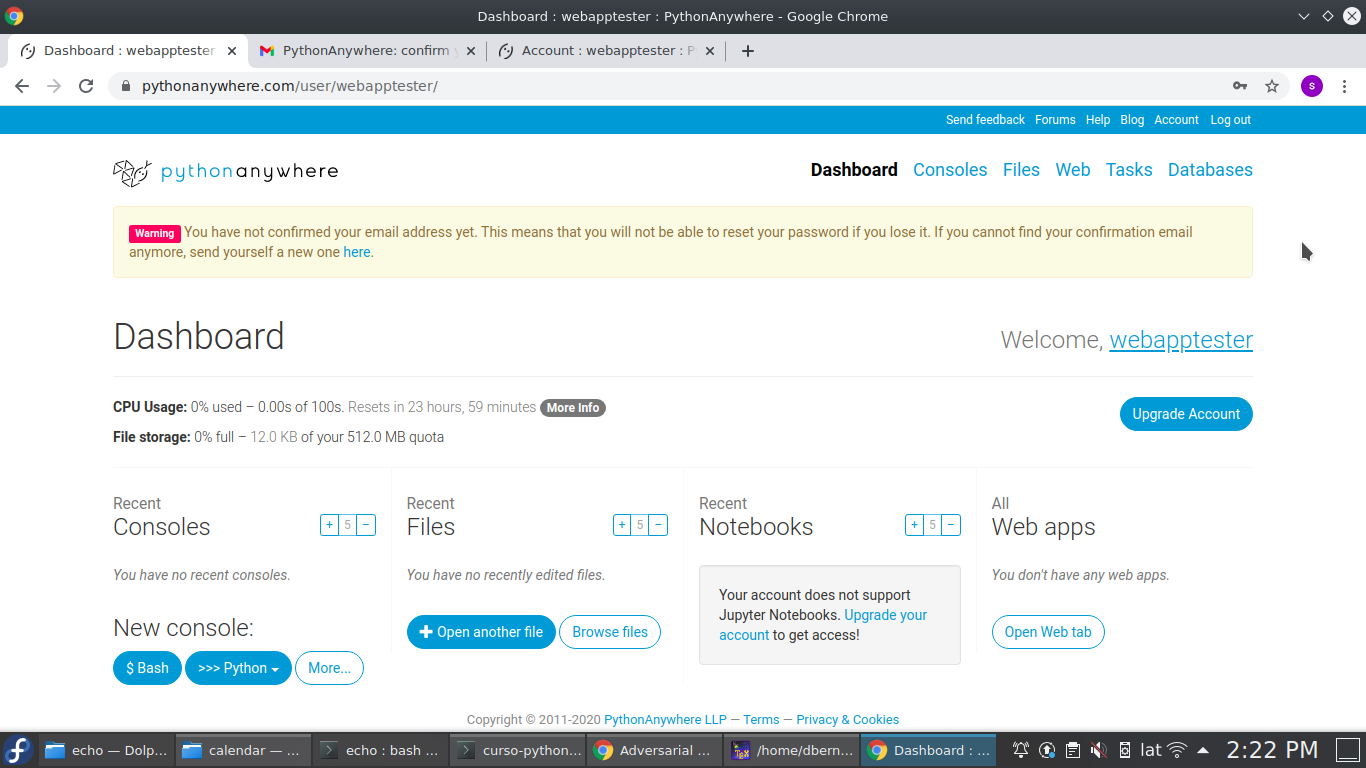
\includegraphics[width=0.7\linewidth]{sc/webapp_dashboard}
	\caption{En Dashboard hay un enlace a la pantalla Web}
	\label{fig:webappdashboard}
\end{figure}

\begin{figure}
	\centering
	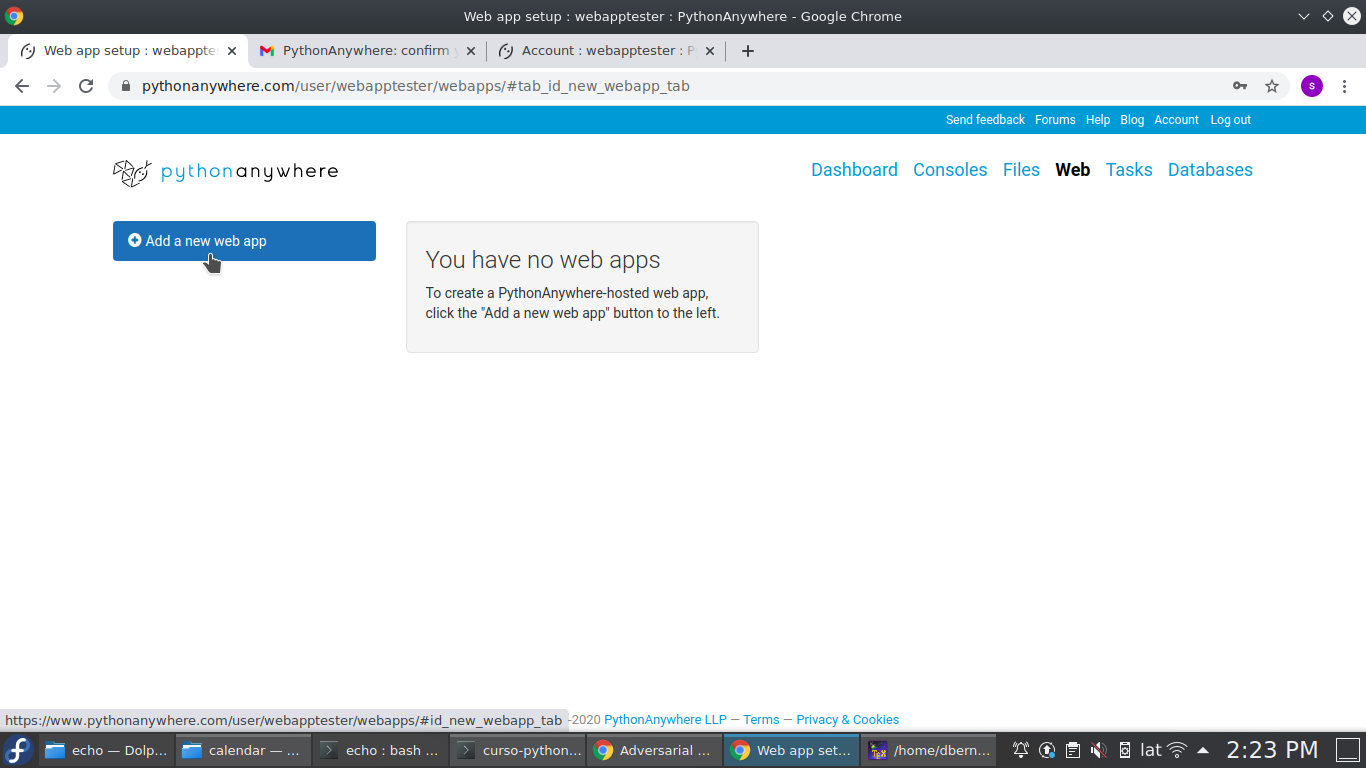
\includegraphics[width=0.7\linewidth]{sc/webapp_create}
	\caption{Aquí podemos crear una apliación web.}
	\label{fig:webappcreate}
\end{figure}

\begin{figure}
	\centering
	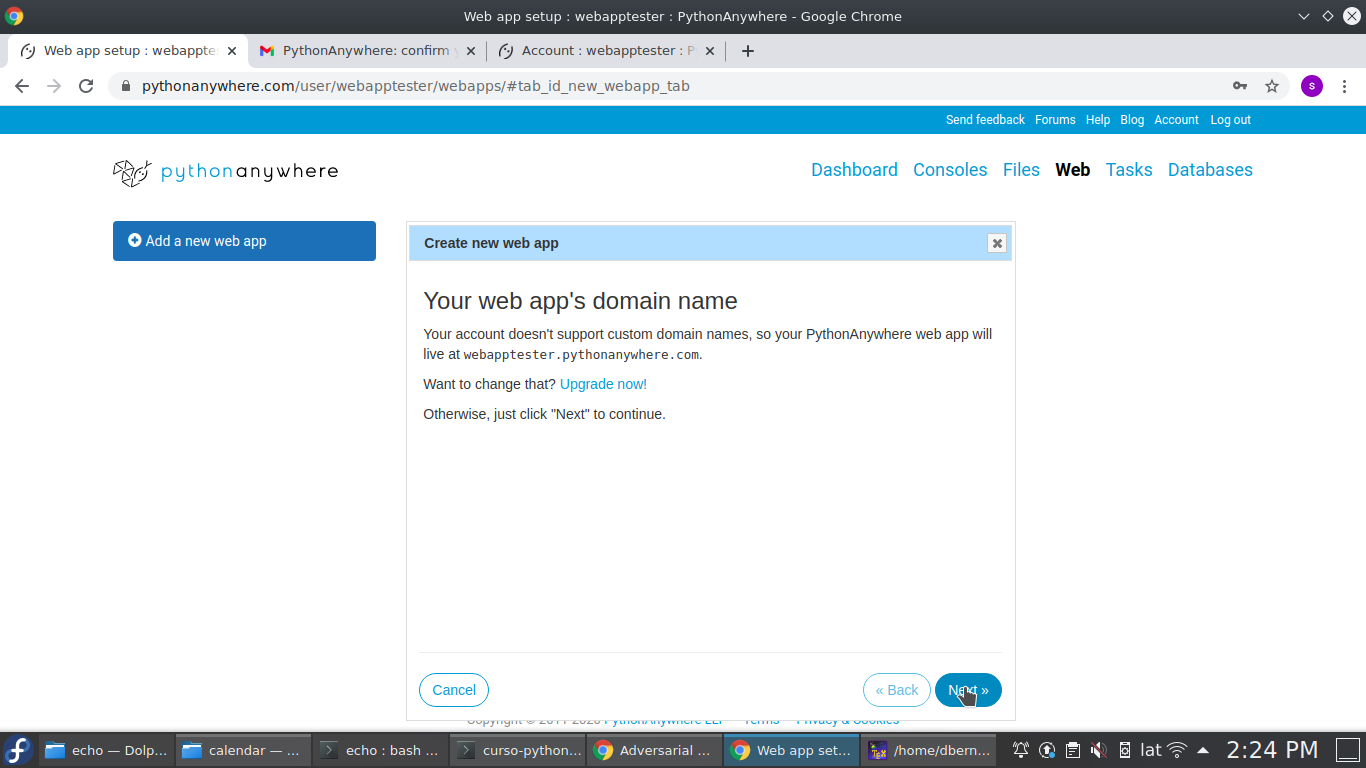
\includegraphics[width=0.7\linewidth]{sc/webapp_domain}
	\caption{Dominio por defecto}
	\label{fig:webappdomain}
\end{figure}

\begin{figure}
	\centering
	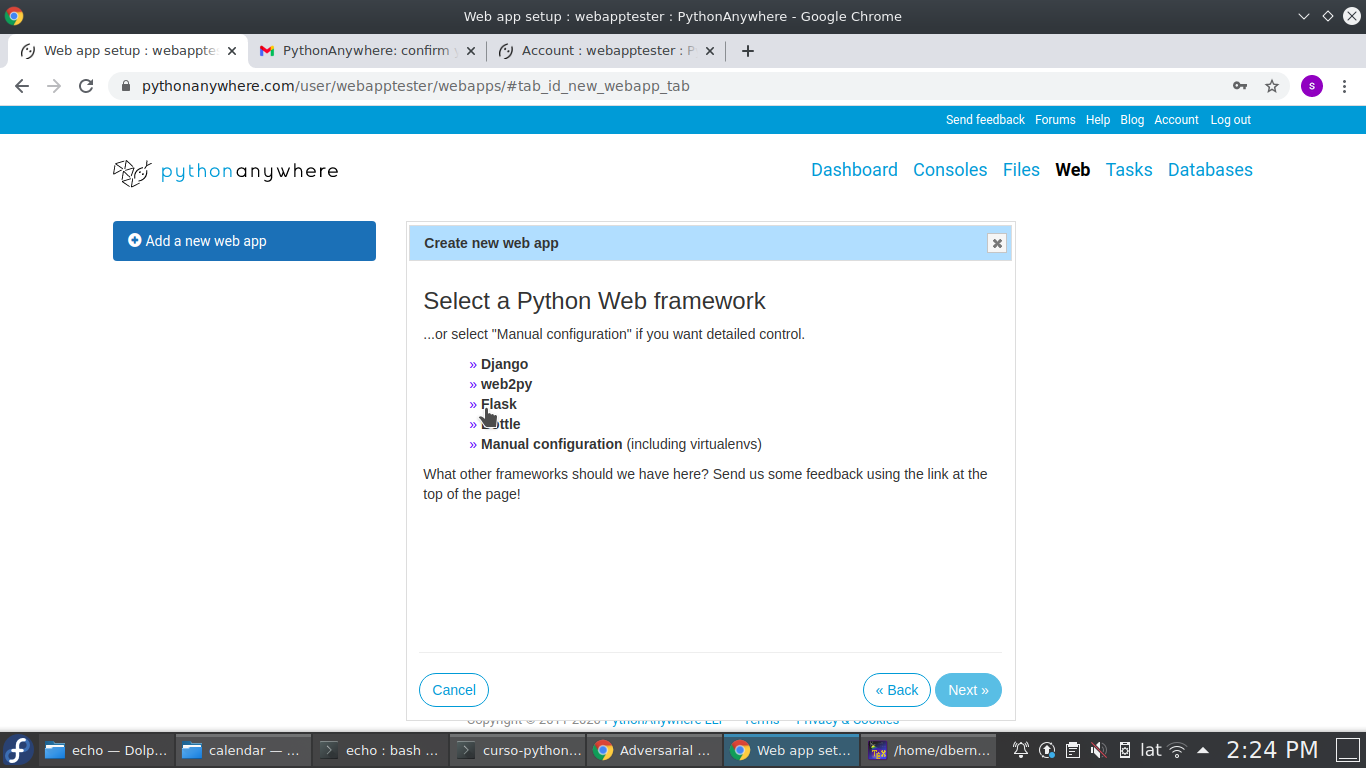
\includegraphics[width=0.7\linewidth]{sc/webapp_flask}
	\caption{Seleccionamos Flask}
	\label{fig:webappflask}
\end{figure}


\begin{figure}
	\centering
	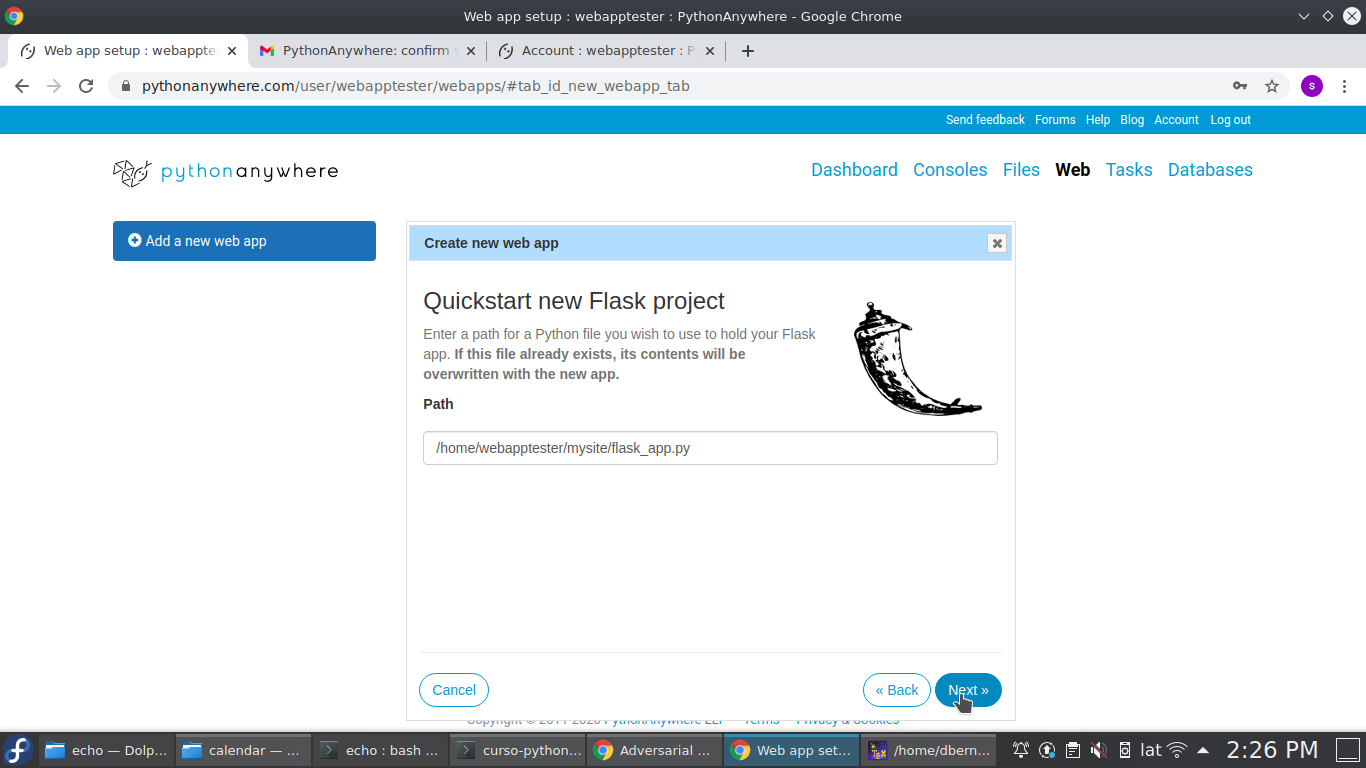
\includegraphics[width=0.7\linewidth]{sc/webapp_mysite}
	\caption{Aceptamos opciones por defecto}
	\label{fig:webappmysite}
\end{figure}

\begin{figure}
	\centering
	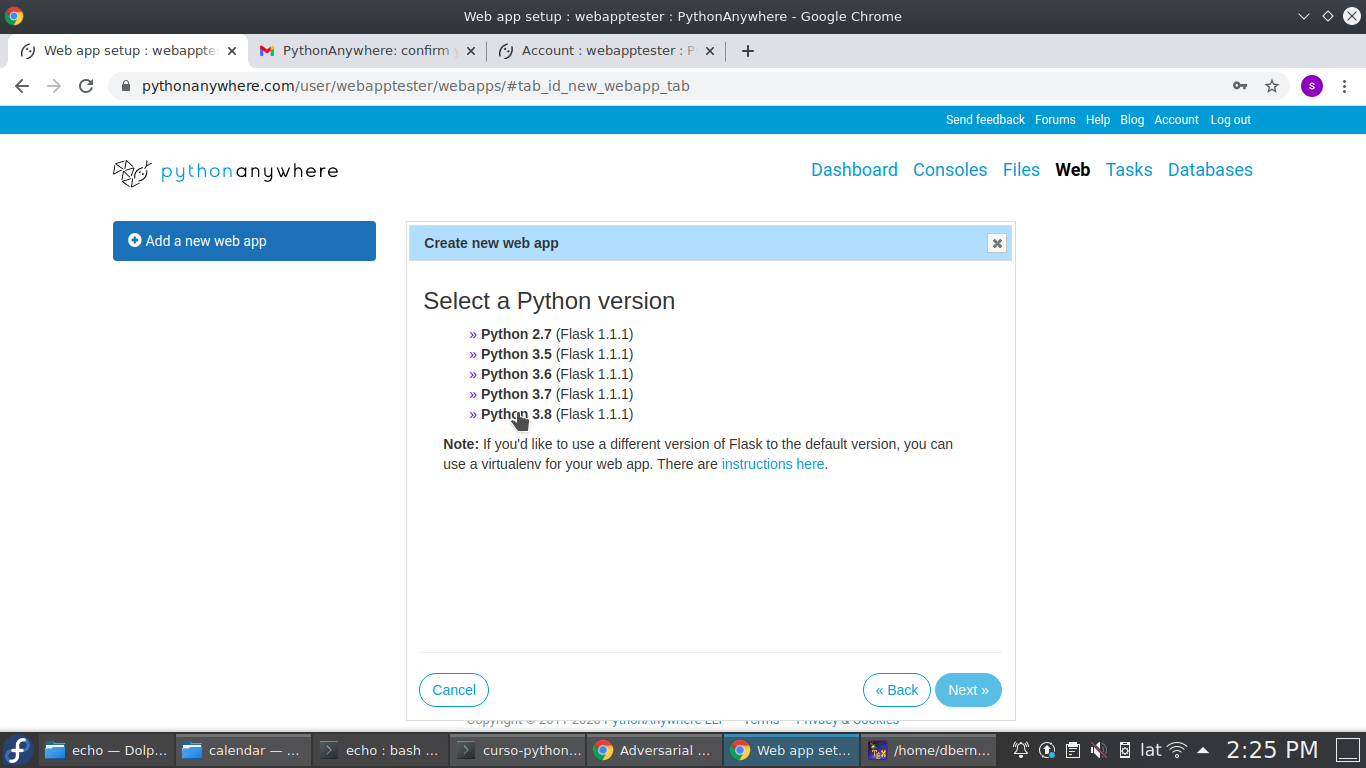
\includegraphics[width=0.7\linewidth]{sc/webapp_python_3_8}
	\caption{Versión de python}
	\label{fig:webapppython38}
\end{figure}

Por ahora aceptamos el dominio por defecto (figura \ref{fig:webappdomain}), seleccionamos Flask (figura \ref{fig:webappflask}), aceptamos el nombre por defecto del sitio web (figura \ref{fig:webappmysite}) y la versión de python (figura \ref{fig:webapppython38}).


En las pantallas (\ref{fig:webapppart1}), (\ref{fig:webapppart2}), (\ref{fig:webappstatic0}), (\ref{fig:webappcode}) vemos distintas partes del panel de control de la aplicación web. Para entender que es lo que estamos haciendo, tenemos que tener en cuenta que un sitio web o aplicación web tiene dos tipos de archivos: dinámicos y estáticos. La aplicación web recibe pedidos en distintas direcciones web o url (universal resource locator), y según los distintos pedidos y 
diferentes urls contesta con archivos dinámicos (generados con información de una base de datos o resultado de algún cálculo) o con archivos estáticos (cuyo contenido es inalterable). 

En el repositorio, en \verb|curso-python/pythonanywhere/calendar|, tenemos un directorio calendars con archivos html conteniendo los calendarios de los años 1900 al 2099. Estos
archivos son inalterables (los calendarios no cambian), por lo tanto los vamos a publicar como archivos estáticos aprovechando que pythonanywhere nos permite definir los archivos con los que responde el servidor web cuando recibe determinados pedidos en ciertas urls (ver figura \ref{fig:webappstatic0}).

\begin{figure}
	\centering
	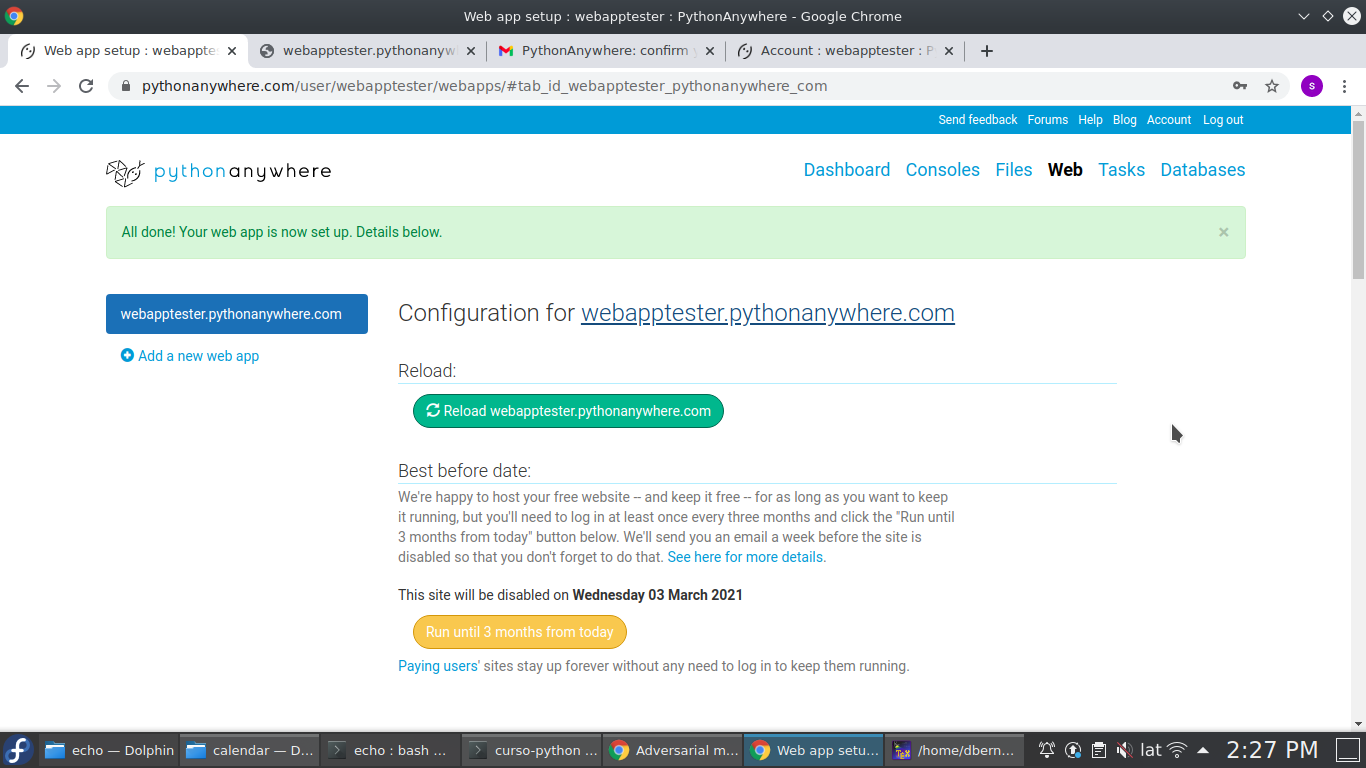
\includegraphics[width=0.7\linewidth]{sc/webapp_part_1}
	\caption{Panel de control de la aplicación web, parte 1}
	\label{fig:webapppart1}
\end{figure}

\begin{figure}
	\centering
	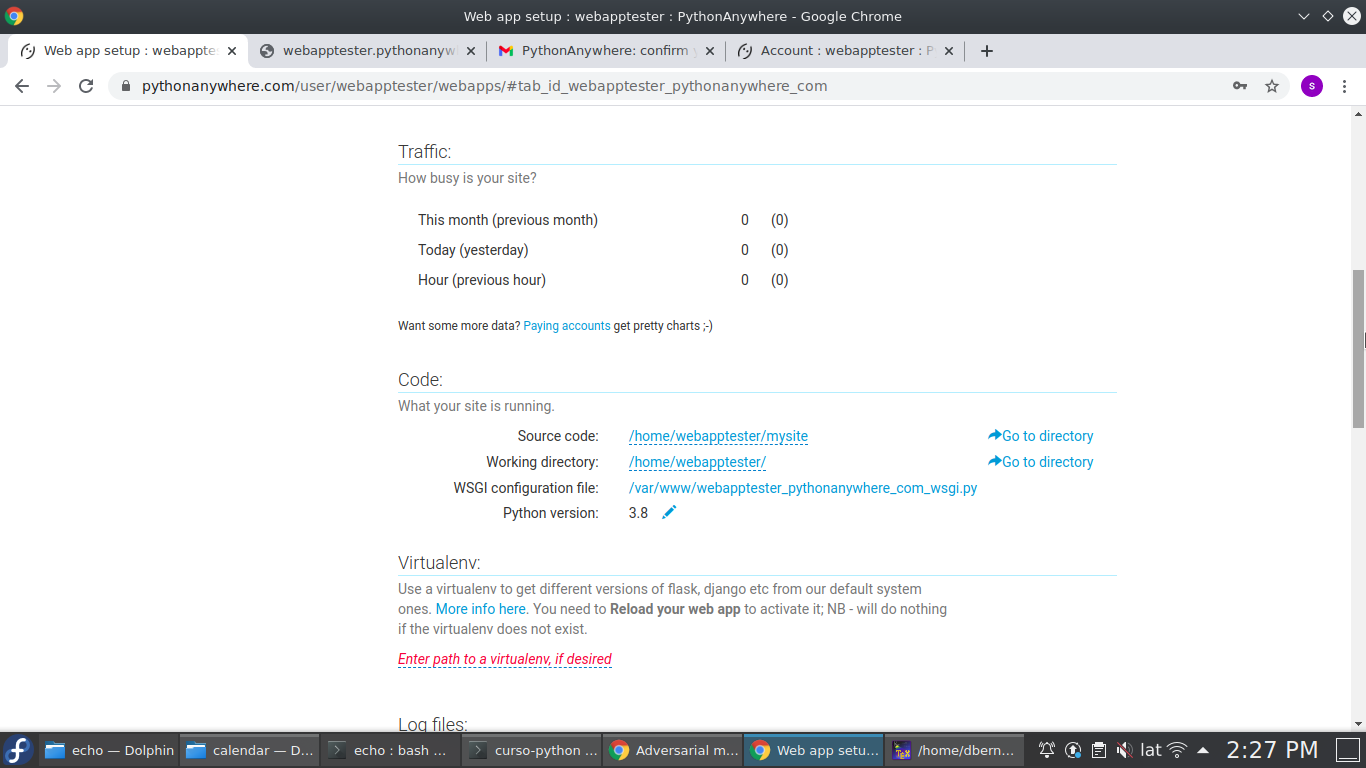
\includegraphics[width=0.7\linewidth]{sc/webapp_part_2}
	\caption{Panel de control de la aplicación web, parte 2}
	\label{fig:webapppart2}
\end{figure}

\begin{figure}
	\centering
	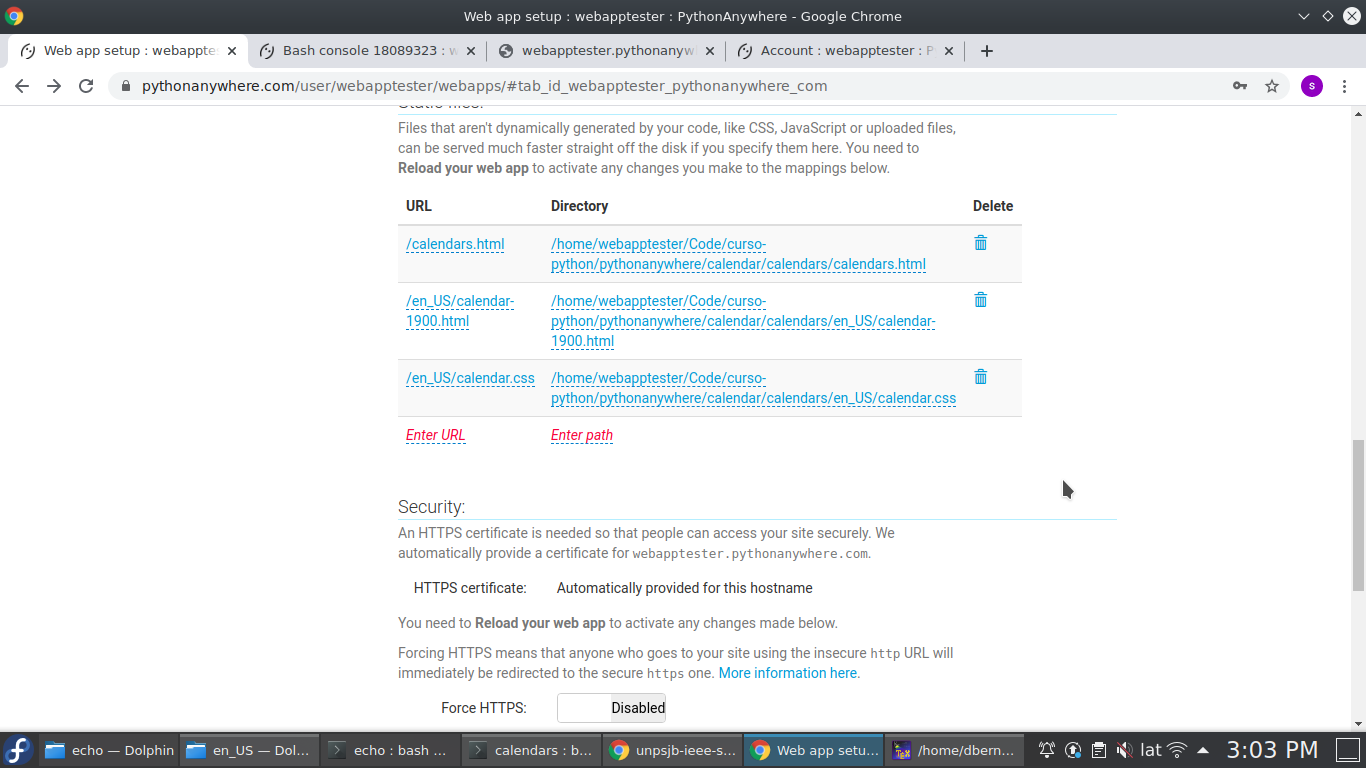
\includegraphics[width=0.7\linewidth]{sc/webapp_static_0}
	\caption{Panel de control de la aplicación web, archivos estáticos}
	\label{fig:webappstatic0}
\end{figure}

\begin{figure}
	\centering
	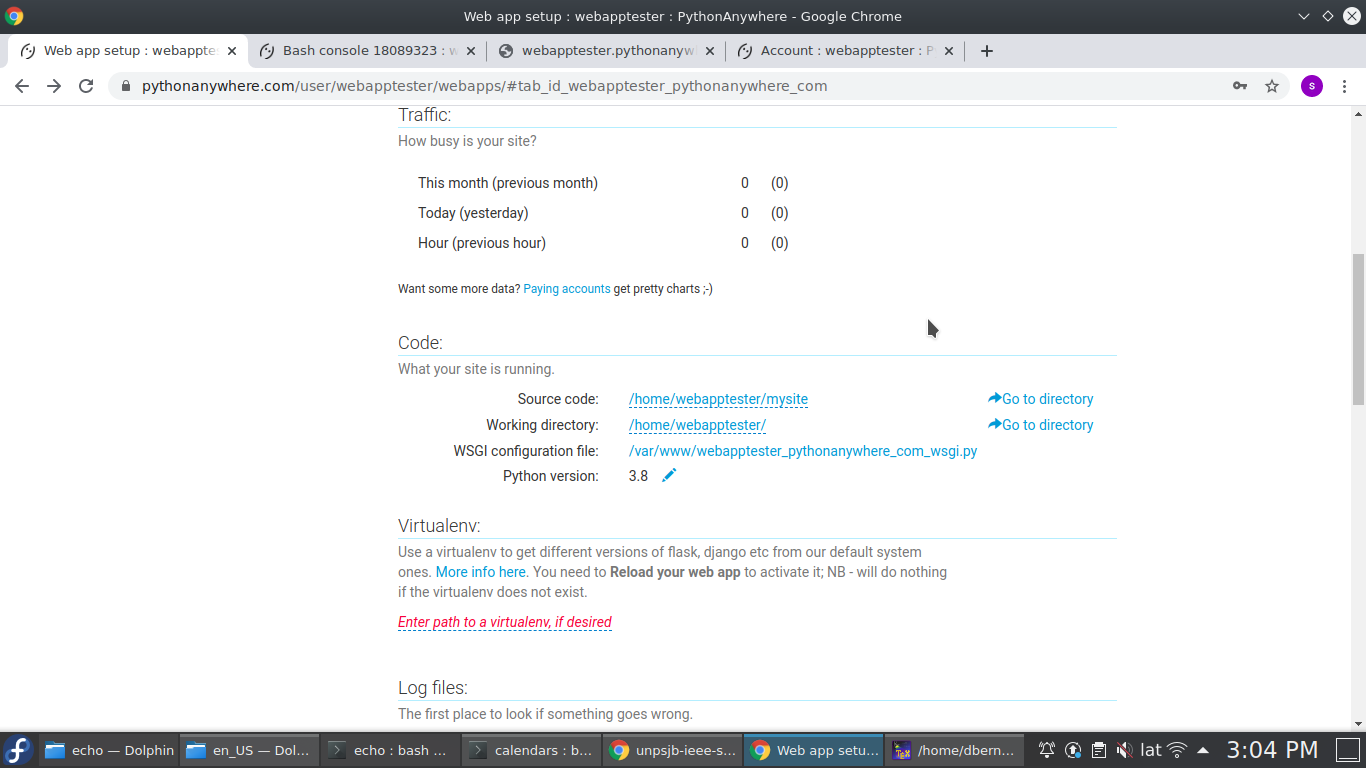
\includegraphics[width=0.7\linewidth]{sc/webapp_code}
	\caption{Panel de control de la aplicación web, donde está el código}
	\label{fig:webappcode}
\end{figure}



\end{document}